\begin{savequote}[8cm]
\textlatin{Cor animalium, fundamentum e\longs t vitæ, princeps omnium, Microco\longs mi Sol, a quo omnis vegetatio dependet, vigor omnis \& robur emanat.}

The heart of animals is the foundation of their life, the sovereign of everything within them, the sun of their microcosm, that upon which all growth depends, from which all power proceeds.
  \qauthor{--- William Harvey \cite{harvey_exercitatio_1628}}
\end{savequote}


\chapter{\label{app:1-sims}PIC simulations}

\minitoc

\section{Convergence of 3D PIC simulations}\label{sec:app-pic_convergence3D}
To reduce the computation cost of the large 3D simulations, a lower resolution version of the original 3D simulation was performed. Results are presented in figure \ref{fig:zvp3dcomparelowres}, demonstrating reasonable convergence.
\begin{figure}
	\centering
	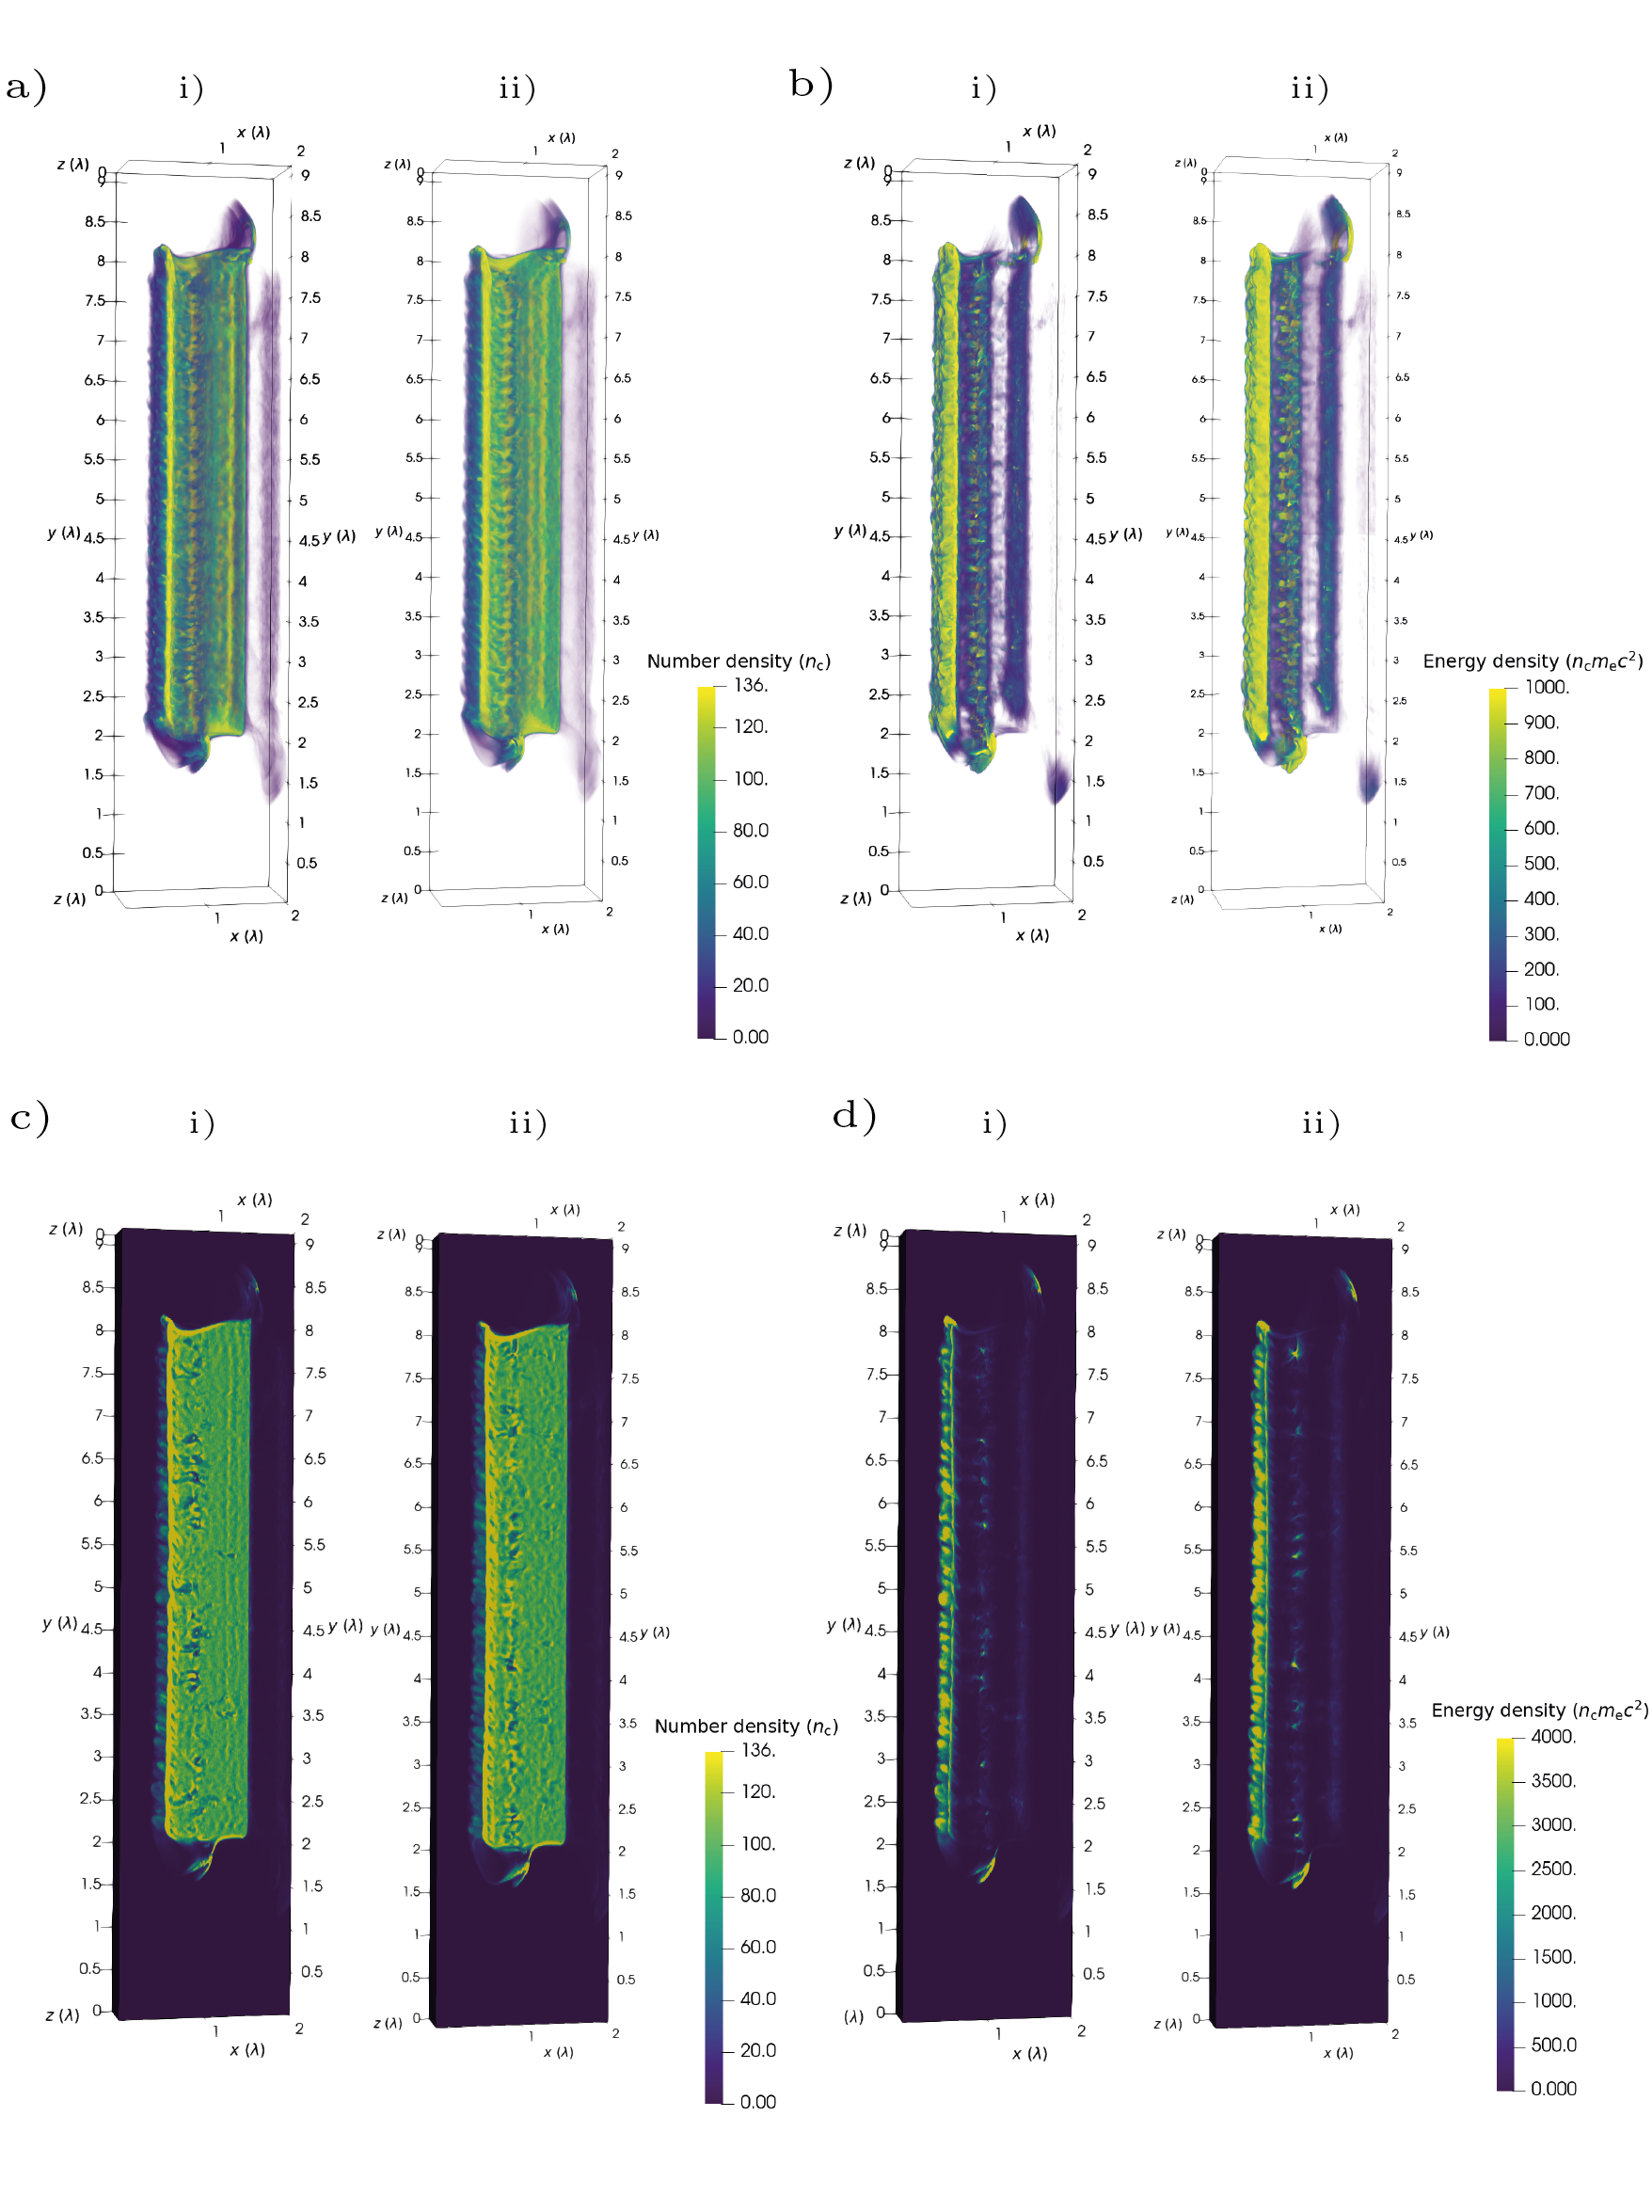
\includegraphics[width=1\linewidth]{figures/zvp/zvp_3D_compare_lowres}
	\caption[Comparison between the initial 3D simulation and a lower resolution version.]{Comparison between the initial 3D simulation and a lower resolution version. a) Electron number density. b) Kinetic energy density. c) and d) are slices of a) and b) respectively. $i$) Initial simulation. $ii$) Lower resolution simulation. Good convergence is demonstrated.}
	\label{fig:zvp3dcomparelowres}
\end{figure}
